\documentclass[a4paper]{article}
\usepackage{tikz}
\usepackage[a4paper,margin=0.5cm]{geometry}
\usepackage{textcomp}

\newcommand{\sometext}{
sol\textbullet{}ami\textbullet{}x meerrettich in apfelessig\textbar raifort au vinaigre de pomme\\
meerrettich, apfelessig, salz, zucker\textbar raifort, vinaigre, sel, sucre\\
abgefüllt\textbar mise en pot 02.06.23 christian@ramseyer.it\\
kühl lagern, sollte einige wochen haltbar sein\textbar
à conserver au frais, peut se conserver pendant plusieurs semaines
}

\begin{document}

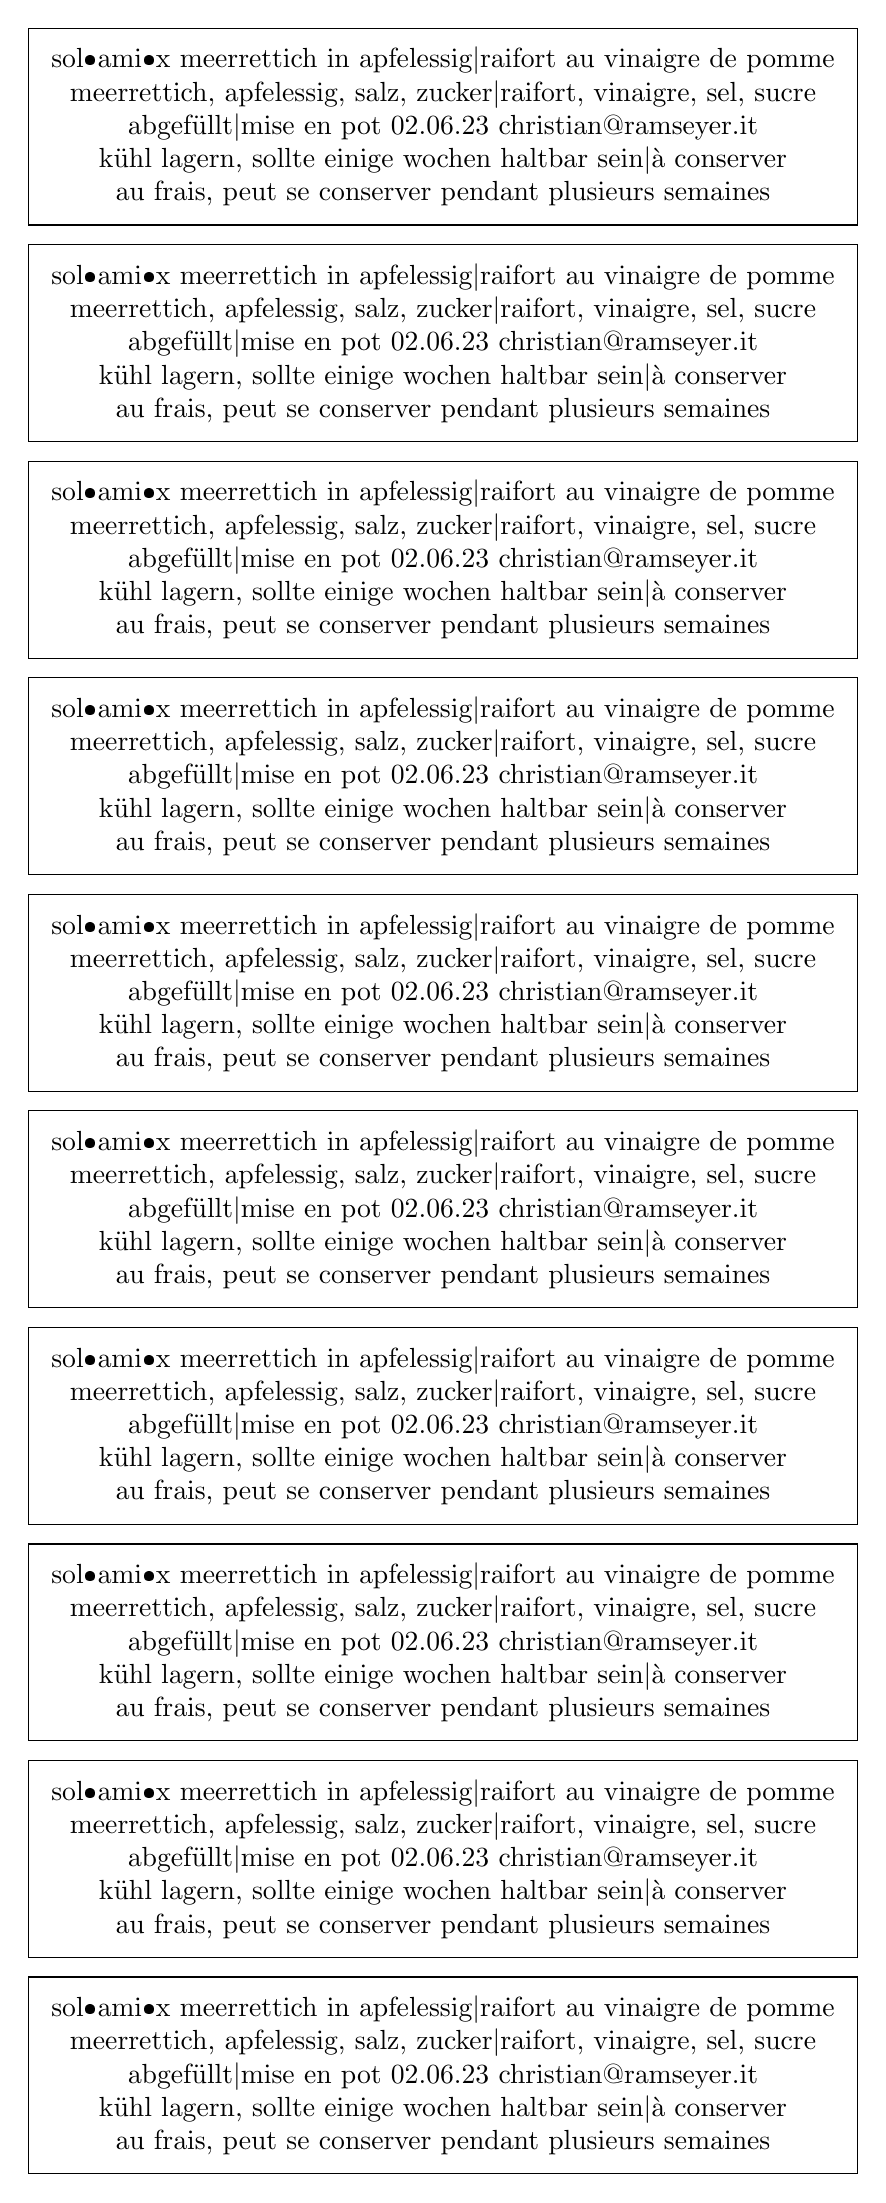
\begin{tikzpicture}
    \foreach \j in {0,...,9} {
        \node[rectangle, minimum width=10.5cm, minimum height=2.5cm, draw, text width=10.3cm, align=center] at (5.25, 2.75*\j+1.25) {\sometext};
    }
\end{tikzpicture}

\end{document}
